\documentclass[11pt,oneside,a4wide]{report}

\usepackage[ngerman]{babel}
\usepackage{graphicx}
\usepackage[svgnames,table,hyperref]{xcolor}
\usepackage{amssymb}
\usepackage{mathtools}
\usepackage{setspace}
\usepackage{listings}
%\usepackage[hyperindex,hidelinks]{hyperref}
\usepackage[hyperindex]{hyperref}

\onehalfspacing

\lstdefinestyle{customXML}{
    belowcaptionskip=1\baselineskip,
    breaklines=true,
    frame=L,
    xleftmargin=\parindent,
    language=XML,
    showstringspaces=false,
    basicstyle=\footnotesize\ttfamily,
    keywordstyle=\bfseries\color{green!40!black},
    commentstyle=\itshape\color{purple!40!black},
    identifierstyle=\color{blue},
    stringstyle=\color{orange},
    numbers=left,
    numberstyle=\tiny,
}
\lstdefinestyle{customSQL}{
    belowcaptionskip=1\baselineskip,
    breaklines=true,
    frame=L,
    xleftmargin=\parindent,
    language=SQL,
    showstringspaces=false,
    basicstyle=\footnotesize\ttfamily,
    keywordstyle=\bfseries\color{green!40!black},
    commentstyle=\itshape\color{purple!40!black},
    identifierstyle=\color{blue},
    stringstyle=\color{orange},
    numbers=left,
    numberstyle=\tiny,
}
\lstdefinestyle{customHTML}{
    belowcaptionskip=1\baselineskip,
    breaklines=true,
    frame=L,
    xleftmargin=\parindent,
    language=HTML,
    showstringspaces=false,
    basicstyle=\footnotesize\ttfamily,
    keywordstyle=\bfseries\color{green!40!black},
    commentstyle=\itshape\color{purple!40!black},
    identifierstyle=\color{blue},
    stringstyle=\color{orange},
    numbers=left,
    numberstyle=\tiny,
}

\newcommand{\HRule}{\rule{\linewidth}{0.5mm}}

\begin{document}

\begin{titlepage}
    \begin{center}

    % Title
    \HRule \\[0.4cm]
    { \huge \bfseries PIM L"osungen\\"Ubung\\[0.4cm] }
    \HRule \\[1.5cm]

    \textbf{Achtung: Dies ist keine offizielle L"osung!}

    \vfill
    Von:\\
    Dustin Wind


   \vfill
    Zuletzt modifiziert am:\\
    {\large \today}\\
    \end{center}
    \bigskip

    {\small
    Bentuzte Software:
    \begin{itemize}
        \item \href{http://www.latex-project.org}{\LaTeX{}: structured text formatting and typesetting}
        \item \href{https://wiki.gnome.org/Apps/Dia/}{Dia: a diagram drawing program}
    \end{itemize}
    }

\end{titlepage}

%\maketitle

\tableofcontents

%\include{inc/Test/test}


\chapter{Aufgabenblatt 01}
\section{Lastenheft}
Da auch die Hochschule mit der Zeit gehen und ihre Studenten bestm¨oglich infomrieren will hat der Dekan beschlossen, eine mobile Applikation entwickeln zu lassen.
Als erstes Modul soll ein Mensa-Informations-System erstellt werden.
Umd die Anwendung in das Budget der Universit¨at einplanen zu k"onnen, bittet man Ihre Abteilung um ein Angebot.\\

\noindent
Sie arbeiten als Software Architekt in der IT-Abteilung der Universit¨at.
Ihr Chef bittet Sie, das vom Dekan erstellte Dokument in ein Anforderungsdokument zu "uberf"uhren.

\subsection{Aufgabe 1: Anforderungsanalyse}
Analysieren Sie das Dokument und "uberlegen Sie sich, ob es m"oglich ist, auf Basis dieser Beschreibung ein Angebot zu erstellen:
\begin{enumerate}
    \item Die Anwendung soll einfach und intuitiv zu bedienen sein und der Gro"steil der Studenten soll sie nutzen k"onnen
    \item Es ist wichtig, dass die Software ansprechend gestaltet ist und den Studenten das Leben vereinfacht
    \item Die App soll die jeweiligen Mensa-Standorte anzeigen k"onnen
    \item Es soll m"oglich sein, die Gerichte der Mensa zu bewerten
    \item Es soll m"oglich sein, wichtige Informationen zur Mensa anzeigen zu lassen
\end{enumerate}

\textbf{L"osung:}
\begin {enumerate}
    \item Die Begriffe "`einfach"',"´intuitiv"',"´Gro"steil"' sind nicht genau spezifiziert, somit nicht SMART- konform
    \item Die Begriffe "´ansprechend gestaltet"' und "´das Leben vereinfacht"' sind nicht genau spezifiziert
    \item Diese Anforderung passt so, wie sie ist
    \item Diese Anforderung passt ebenfalls
    \item Der Begriff "´wichtige Informationen"' sollte n"aher spezifiziert sein
\end{enumerate}
    
\subsection{Aufgabe 2: Erstellung Anforderungsdokument}
Um den Dekan bestm"oglich zu unterst"utzen, erstellen Sie einen Vorschlag f"ur ein detailliertes Anforderungsdokument, das als Grundlage f"ur die sp"atere Entwicklung dienen soll. 
Bitte nutzen Sie dazu die vom Dekan gemachten Angaben als Basis.

\textbf{L"osung:}
\begin{enumerate}
    \item Die app soll eine Einstiegsseite mit einem "Uberblick "uber die Funktionen der App bieten 
    \item Es soll eine Karte mit den relevanten Mensa- Standorten eingebunden werden, welche eine Navigationsm"oglichkeit enth"alt 
    \item Es soll ein Mensa- Modul enthalten sein, welches den Speiseplan und Bewertungsfunktionen enth"alt 
    \item Eine Anbindung an das UNIVIS soll vorhanden sein 
    \item Es soll m"oglich sein, den eigenen Vorlesungsplan zu hinterlegen
    \item E- Learning- Inhalte sollen integriert sein 
    \item "Uber eine Facebook- Anbindung sollen Community-Features inkl. Diskussionsforum realisiert werden 
    \item Das Projekt soll durch Werbung finanziert werden 
    \item Eine Anzeige von Veranstaltungen des t"aglichen Studentenlebens soll m"oglich sein
\end{enumerate}




\chapter{Aufgabenblatt 02}

\section{HTML}
Sie sind weiterhin mit der Erstellung des Mensa Moduls f"ur die mobile Anwendung der Universit"at beauftragt.
Mittlerweise wurde entschieden, die Anwendung in Form einer mobilen Webseite zu implementieren.
Um sich mit HTML vertraut zu machen versuche Sie, die folgende Struktur als HTML Seite umzusetzen.

\subsection{Erstellung eines HTML-Dockuments}
Erstellen Sie ein neues HTML Dokument mit dem nahem "`MensaApp.html"':
\begin{itemize}
    \item Seitentitel: "`MensaApp"'
    \item "Uberschrift $h1$: "`MensaApp der FAU""
    \item Einf"uhrender Text: "`Herzlich Willkommen auf der Startseite"' in fetter Schrift
    \item Freitext in neuem Absatz: "`Als Student haben Sie die M"oglichkeit an folgenden Mensen zu speisen:"'
    \item Ungeordnete Liste mit folgenden Eintr"agen:
    \begin{itemize}
        \item Mensa Langemarckplatz
        \item S"udmensa
        \item Mensa Insel Sch"utt
        \item Mensa Regensburger Stra"se
        \item Ausgabemensa St. Paul
        \item Mensateria Ohm
    \end{itemize}
    \item Die einzelnen Eintr"age sollen auf die jeweiligen Links zu den entsprechenden Speisepl"anen verweisen, welche hier zu finden sind: \url{http://www.studentenwerk.uni-erlangen.de/verpflegung/de/speiseplaene.shtml}
    \item Pr"ufen Sie das HTML Dokument, indem Sie es sich im Browser anzeigen lassen
\end{itemize}

\lstset{style=customHTML}
\lstinputlisting[style=customHTML]{./inc/aufgabe02/mensaapp.html}



\chapter{Aufgabenblatt 03}


\section{Datenmodellierung}

\subsection{Aufgabe 1: ERM}

Ihnen liegt der nachfolgende Auszug aus dem Pflichtenheft vor. Bitte "uberf"uhren Sie diesen in ein Entity-Relationship-Diagramm mit Chen Notation.
Bestimmen Sie dazu die relevanten Entity-Typen, deren Beziehung untereinander soweie deren Kardinalit"aten und Attribute.
Bestimmen Sie daraufhin die jeweiligen Schl"usselattribute.\\

\textbf{Auszug aus dem Pflichtenheft}
\begin{itemize}
    \item Jede Mensa ist eindeutig durch einen Namen, Ort und eine Dienststellennummer charakterisiert und wird durch einen Mensa-Chef geleitet.
    Dieser besitzt neben seinem Namen und Vornamen auch eine Personalnummer und einen Rang.
    Es kann auch m"oglich sein, dass der Chef f"ur mehr als eine Mensa Zust"andig ist.
    \item Jede Mensa bietet verschiedene Gerichte an.
    Es handelt sich dabei entweder um dauerhafte Angebote oder ein saisonales "`Special"'.
    Um die Zuordnung zu vereinfachen besitzt jedes der Gerichte eine interne Referenznummer, einen Namen und eine Beschreibung.
    Es kann sich dabei sowohl um eine Vor-, Haupt-, oder Nachspeise handeln.
    Die Gerichte haben dar"uber hinaus eine Bewertung, welche die Beliebtheit bei den Studenten widerspiegeln soll.
    Mede Mensa bietet zu unterschiedlichen Zeitpunkten unterschiedliche Gerichte an.
    \item Jedes der Gerichte besteht aus einer oder mehreren Zutaten.
    Diesen sind durch eine Bestelnummer und die Bezeichnung gekennzeichnet.
    Dar"uber hinaus dienen der Haltbarkeitszeitraum, die Angabe der m"oglichen Allergika sowie die Angabe ob vegetarisch oder nicht als wichtige Informationen.
\end{itemize}

\bigskip
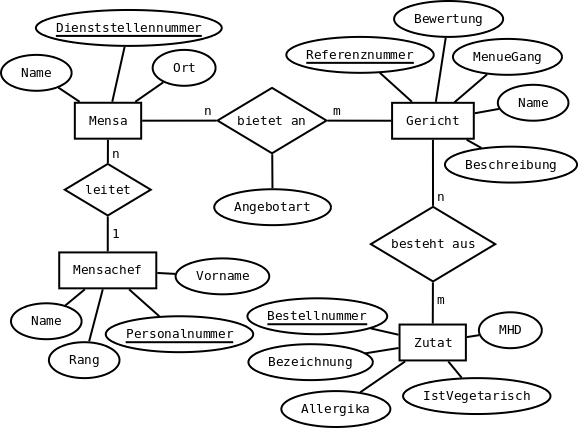
\includegraphics[scale=0.5]{./inc/aufgabe03/mensaapp.png}

\subsection{Aufgabe 2: Relationenschema}
"Uberf"uhren Sie nun das von Ihnen erstelte ERM-Diagramm in das Relationenmodell.\\

\noindent
\fbox{
    \parbox{\textwidth}{
        \textbf{Mensachef}(\underline{Personalnummer}, Name, Vorname, Rang)\\
        \textbf{Mensa}(\underline{Dienststellennummer, Name, Ort}, $\overline{Personalnummer}$)\\
        \textbf{Gericht}(\underline{Referenznummer}, Name, Beschreibung, Angebotart, MenueGang, Bewertung, $\overline{Mensa}$)\\
        \textbf{Zutat}(\underline{Bestellnummer}, Bezeichnung, MHD, Allergika, IstVegetarisch)\\
        \textbf{Rezept}(\underline{GerichtId[Gericht], ZutatId[Zutat]})\\
        
        \noindent
        {\small \textbf{Anm. des Autors}: Fremdschl"usselbeziehungen k"onnen entweder durch einen Oberstrich gekennzeichnet werden, oder durch das Angeben der Tabelle, auf die der  Fremdschl"ussel refenziert, in eckigen Klammern.\\
        Im Zweifel sollte w"ahrend der Klausur die Methode der Vorlesung gew"ahlt werden!}
    }
}




















\chapter{Aufgabenblatt 04}

\section{Datengest"utzte Anwendungen}
In der vergangenen Woche haben Sie das Relationenmodell f"ur die mobile Uni-Applikation erstellt.
Dies liegt mittlerweile in der Datenbank vor.
F"ur die Entwicklung des Mensa-Moduls ben"otigen Sie Ausschnitte aus dieser Datenbank f"ur die Anzeige auf dem mobilen Client.\\
In der Vorlesung haben Sie die Elemente von SQL-Abfragen kennen gelernt.


\subsection{Aufgabe 1: SQL}
Erstellen Sie eine Abgrage, die den Namen und die Bewertung aller Gerichte ausgibt, die in der Zentralmensa in N"urnberg angeboten werden.

\lstset{style=customSQL}
\begin{lstlisting}
SELECT      g.Name, g.Bewertung
FROM        Gericht AS g
            JOIN Speiseplan AS s ON g.Referenznummer = s.GerichtId
            JOIN Mensa AS m ON s.MensaId = m.Dienststellennummer
WHERE       m.Ort = 'Nuernberg'
            AND m.Name LIKE '%Zentralmensa%'
;
\end{lstlisting}

\subsection{Aufgabe 2: SQL}
Listen Sie den Namen und die Beschreibung aller vegetarischen Gerichte auf, die in den Mensen des Studentenwerks angeboten werden.
Beachten Sie dabei, dass ein Gericht nur dann vegetarisch ist, wenn alle Zutaten vegetarisch sind.\\

\lstset{style=customSQL}
\begin{lstlisting}
SELECT      Name, Beschreibung
FROM        Gericht
WHERE       Gericht.RefNum NOT IN
            (
                -- create a table with all meals containing meat
                SELECT      r.GerichtID
                FROM        Rezept AS r
                            LEFT OUTER JOIN 
                            (
                                SELECT  z.BestNum
                                FROM    Zutat AS z
                                WHERE   z.IstVegetarisch = 1
                            ) AS x
                            ON r.ZutatId = x.BestNum
                -- due to the left-outer join all 
                -- meat-containing meals in table r join x
                -- have their column 'BestNum' set to NULL
                WHERE       x.BestNum IS NULL
            )
;
\end{lstlisting}



\noindent
Beispiel-Tabelle (Rezept):\\
\rowcolors{1}{LightGrey}{White}
\begin{tabular}{ l l }
    \rowcolor{LightSlateGray}
    \textbf{GerichtId}  & \textbf{ZutatId}\\
    id(Currywurst)      & id(Wurst)\\
    id(Currywurst)      & id(Curry)\\
    id(Kartoffelpuffer) & id(Kartoffeln)\\
    id(Kartoffelpuffer) & id(Apfelmus)\\
\end{tabular}






\chapter{Aufgabenblatt 05}

\section{ User Experience and Usability }
Das  von  Ihrer  IT  Abteilung  zu  entwickelnde  mobile  Universit"ats-Portal  dient  vorwiegend  der Nutzung  durch  Studenten.  
Jedoch  auch  f"ur  die  Bediensteten  der  Hochschule  bieten  sich dadurch  zahlreiche  Vorteile.  
In  der  Vorlesung  haben  Sie  Methoden  des  Prototyping, Storytelling sowie die Erstellung von Personas kennengelernt. 


\subsection{Aufgabe 1: Personas}
Im  Rahmen  der  Usability  Methoden  haben  Sie  neben  der  Nutzergruppendefinition  das Konstrukt der Personas kennengelernt.  
Bitte erstellen Sie insgesamt vier Personas, davon jeweils zwei f"ur die Gruppe der Studenten sowie zwei f"ur die Gruppe der Bediensteten. 

\textbf{L"osung:}
\begin{itemize}
    \item Student 1 : Max Mustermann\\
        M"annlich, studiert im 3. Semester Maschinenbau.
        Mag vornehmlich fleischlastige und deftige Speisen, m"ochte schnell und g"unstig in seiner Mittagspause etwas essen.
        Hat nicht den Willen, beim Essen am Handy zu sein und w"ahrenddessen sozial zu interagieren.
        Das Essen ist f"ur ihn eher Mittel zum Zweck als eine T"atigkeit, mit der er sich auseinander setzt.
    \item Student 2 : Martina Mustermann\\
        Weiblich, studiert im 5. Semester Gender Studies.
        Vegan aus "Uberzeugung, w"ahlt ihr Essen bewusst aus und setzt sich intensiv mit ihrer Nahrungsaufnahme auseinander.
        Interagiert st"andig sozial, bewertet gerne Produkte online und schreibt Rezensionen.
    \item Bediensteter 1: Jon Doe\\
        Wie Max, ist blo"s schon fertig mit seiner Ausbildung und 40 Jahre alt. 
    \item Bediensteter 2 : Jennifer Doe\\
        Wie Martina, abgesehen von der Tatsache dass sie 45 Jahre alt ist und mit ihrer Ausbildung fertig.
\end{itemize}

\subsection{Aufgabe 2:  Contextual Inquiry and Storytelling }
Um  die  Bed"urfnisse  der  Nutzer  bestm"oglich  abzudecken  und  damit  eine  erfolgreiche Anwendung zu erstellen ist es unabdingbar, den sp"ateren Nutzungskontext zu kennen.\\
\begin {enumerate}
    \item Bitte beschreiben Sie exemplarisch (2-3 S"atze) den Nutzungskontext f"ur jede der zuvor erstellten  Personas.  
        F"ur  die  Gruppe  der  Studenten  soll  dabei  ein  Interview  mit Kommilitonen dienen, die in der jeweiligen Nutzergruppe liegen.  \\
    \textbf{L"osung:}
    \begin{itemize}
        \item Max: \\
            Er geht in die Mensa mit dem Ziel, schnell satt zu werden und wieder herauszukommen.
            Er m"ochte schnell und g"unstig etwas essen.
            Er hat nicht vor, die App f"ur soziale Interaktion zu nutzen.
        \item Martina: \\
            Sie geht in die Mensa mit dem Ziel, etwas gesundes und "okologisch wertvolles zu essen.
            Sie nimmt sich Zeit zum essen und zahlt auch gerne etwas mehr, falls das Essen ihren Qualit"atsanspr"uchen gen"ugt.
            Sie will die App zum bewerten von Gerichten und zum sozial interagieren verwenden.
        \item Jon: \\
            Wie Max,nur "alter und mit etwas mehr Budget.
        \item Jennifer: \\
            Wie Martina, nur mit mehr Zeit, ausf"uhrlicheren Bewertungen und noch h"oheren Qualit"atsanspr"uchen.
    \end{itemize}
    \item W"ahlen  Sie  zwei  der  erstellten  Personas  aus  und  wenden  Sie  die  Methode  des Storytelling  an.  
        Wie  kann  die  sp"atere  Nutzung  des  Mensa  Moduls  anhand  einer Geschichte erz"ahlt werden? \\
    \textbf{L"osung:}        
    \begin{itemize}
        \item Max: \\
            Max m"ochte in der app schnell die im Moment g"unstigste Mensa finden, die f"ur ihn am schnellsten zu erreichen ist. 
            Hierf"ur sieht er sich zuerst die Mensa- "Ubersicht an und dann die jeweiligen Speisepl"ane. 
            Hat er dies erledigt, benutzt er die App, um sich zur Mensa seiner Wahl navigieren zu lassen. 
        \item Martina: \\
            Martina nutzt die app ausgiebig, um sich "uber die Zutaten der einzelnen Gerichte zu informieren und so das ihr am besten gefallende Gericht zu finden. 
            Sobald sie ein Gericht ausgesucht hat, l"asst sie sich zur entsprechenden Mensa navigieren.
            Beim Essen tauscht sie sich "uber die Community- Features der app mit anderen, in der Mensa anwesenden Personen "uber das Gericht, welches sie gerade isst, aus.
            Sobald sie mit dem Essen fertig ist, verfasst sie eine Rezension und ein gibt ein Rating f"ur das Gericht ab.
    \end{itemize}
\end {enumerate}

\subsection{Aufgabe 3: Prototyping  }
Das  Prototyping  einer  Anwendung  dient  unter  anderem  der  fr"uhzeitigen  Visualisierung  der sp"ateren Anwendung. 
Um Ihr Konzept so bald wie m"oglich anhand der Nutzergruppe validieren zu können entschlie"sen Sie sich, das Mensa Modul als Mockup umzusetzen.  
Erstellen  Sie  dazu  Design- Mockups item Der  Mensa  Startseite, des Speiseplans und der Detailseite eines Gerichts inklusive Bewertungssystem.

\begin{figure}[h]
    \centering
    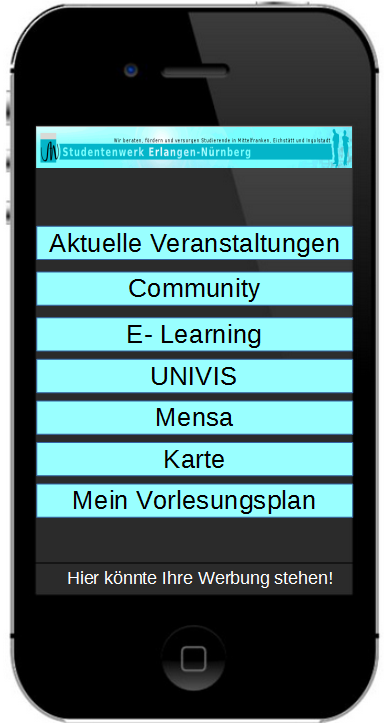
\includegraphics[scale=0.4]{./inc/aufgabe05/MockupStartseite} 
    \caption{Mockup: Startseite}
\end{figure}

\begin{figure}[h]
    \centering
    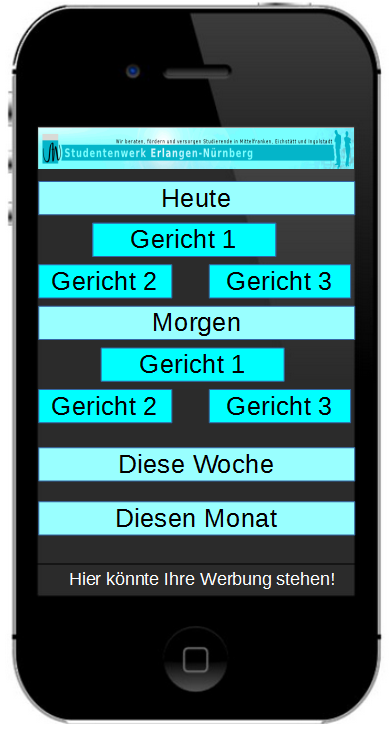
\includegraphics[scale=0.4]{./inc/aufgabe05/MockupSpeiseplan}
    \caption{Mockup: Speiseplan}
\end{figure}

\begin{figure}[h]
    \centering
    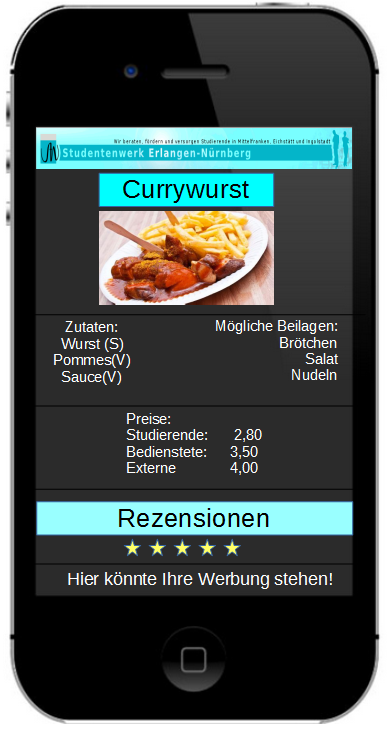
\includegraphics[scale=0.4]{./inc/aufgabe05/MockupGericht}
    \caption{Mockup: Gericht}
\end{figure}










        

    


\chapter{Aufgabenblatt 07}

\section{Datenmodellierung mit XML}
Bestellungen der Mensa sollen innerhalb des E-Procurement-Systems direkt an die Lieferanten weitergeleitet werden.
Die Lieferanten haben dazu jeweils definierte Auftragsschnittellen, die in XML definiert sind.\\

\subsection{Aufgabe 1: XML-Definition}
Bitte erstellen Sie eine XML-Definition (DTD), mit der Bestellung an einen Lieferangen "ubergeben werden und speichern Sie dieses als "`Order.dtd"' ab.
Bitte ber"ucksichtigen Sie dabei die folgenden Anforderungen:
\begin{itemize}
    \item Tag-Namen sind grunds"atzlich in Englisch zu erstellen.
    Die Bestellung (Order) ist das Root-Element.
    \item Jede Bestellung enth"alt Name (SupplierName) und Id (SupplierID) des Lieferanten sowie das Auftragsdatum (OrderDate) und die Auftragsnummer (OrderNumber) als Elemente.
    Eine Bestellung besteht zudem aus mindestens einem Bestellposten (Item).
    \item Jeder Bestellposten bezieht sich auf ein bestimmtes Lebensmittel.
    F"ur das Lebensmittel sollen neben Produktnummer (ItemNumber) sowie der Preis (Price) als Elemente mit angegeben werden.
    Optional ist angegeben, wievielKalorien (Calories) das Nahrungsmittel pro 100g hat.
    \item Der Standard-Lieferant der Mensa, "`Bauernhof Meier"' wird fest im System hinterlegt.
    Bei Eingabe des K"urzels "`BM"' soll dieses automatisch durch die Zeichenkette "`Bauernhof Meier Nuernberg"' ersetzt werden.
\end{itemize}

\noindent
Ob Ihre DTD valide ist k"onnen sie auf folgender Seite "uberpr"ufen:\\
\url{http://www.validome.org/grammar/validate/}\\


\lstinputlisting[style=customXML]{./inc/aufgabe07/order.dtd}

\subsection{Aufgabe 2: XML-Daten}
Bitte erstellen Sie auf Basis der Definition eie XML-Datei (Order.xml), die die DTD referenziert und die mindestens vier Bestellposten enth"alt.
Stellen Sie bitte sicher, dass die erstellte XML Datei sowohl g"ultig als auch wohlgeformt ist.\\

\lstinputlisting[style=customXML]{./inc/aufgabe07/order.xml}

\section{XML/KML und Mashup}
Als besonderes Extra m"ochten Sie in das Mensa Modul Ihres mobilen Universit"atsportals eine Google Maps Karte einbauen.\\

\subsection{Aufgabe 1: Statische Positionsbeschreibung}
Sie m"ochten die Positionen der einzelnen Mensen auf einer Google Maps Karte in der Satellitendarstellung anzeigen lassen.\\
Erstellen Sie dazu eine KML Datei und f"ugen Sie die Positionen der folgenden Mensen als einfache Lokation hinzu:
\begin{itemize}
    \item Mensa Langemarckplatz, Langemarckplatz 4, 91054 Erlangen
    \item S"udmensa, Erwin-Rommel-Stra"se 60, 91058 Erlangen
    \item Mensa Insel Sch"utt, Andreij-Sacharow-Platz 1, 90403 N"urnberg
    \item Mensa Regensburger Stra|se, Regensburger Str. 160, 90478 N"urnberg
    \item Ausgabemensa St. Paul, Dutzendteichstra"se 24, 90478 N"urnberg
    \item Mensateria Ohm, Wollentorstr. 4, 90409 N"urnberg
\end{itemize}
Iin der Beschreibung der Positionen sollen sowohl der name der Mensa als auch die vollst"andige Adresse angezeigt werden.\\
Um die Funktionalit"at der von Ihnen erstellten Datei testen zu k"onnen, kopieren Sie bitte den Quelltext in die Zwischenablage und lassen Sie sich die Karte auf folgender Webseite anzeigen:\\
\url{http://display-kml.appspot.com}

\lstinputlisting[style=customXML]{./inc/aufgabe07/app1.kml}


\subsection{Aufgabe 2: Polygone in KML}
Zus"atzlich zu den Positionen der einzelnen Mensen m"ochten Sie auch die WISO Fakult"at auf der Karte darstellen.
Sie m"ochten die Einrichtung jedoch nicht nur als einfachen Marker darstellen, sondern das Geb"aude farblich markieren.\\
Erweitern Sie dazu im Text Editor die in Aufgabe 1 erstellte KML Datei so, damit sie folgende Eigenschaften zur Darstellung der farblichen Markierung erf"ullt:
\begin{itemize}
    \item Darstelung eines Polygons
    \item Die "au"sere Kante soll entlang der folgenden Koordination verlaufen:
    \begin{itemize}
        \item 11.084944,49.458151,100
        \item 11.085081,49.457841,100
        \item 11.086463,49.458082,100
        \item 11.086058,49.459037,100
        \item 11.084810,49.458803,100
        \item 11.084875,49.458592,100
        \item 11.085661,49.458713,100
        \item 11.085838,49.458312,100
    \end{itemize}
\end{itemize}
Speichern Sie die Datei unter dem Namen mensafak.kml.\\
Um die Funktionalit"at der von Ihnen erstellten Datei testen zu k"onnen, kopieren Sie bitte den Quelltext in die Zwischenablage und lassen Sie sich die Karte auf folgender Webseite anszeigen:\\ 
\url{http://display-kml.appspot.com}


\lstinputlisting[style=customXML]{./inc/aufgabe07/app2.kml}








\end{document}


